\documentclass[english,,man]{apa6}
\usepackage{lmodern}
\usepackage{amssymb,amsmath}
\usepackage{ifxetex,ifluatex}
\usepackage{fixltx2e} % provides \textsubscript
\ifnum 0\ifxetex 1\fi\ifluatex 1\fi=0 % if pdftex
  \usepackage[T1]{fontenc}
  \usepackage[utf8]{inputenc}
\else % if luatex or xelatex
  \ifxetex
    \usepackage{mathspec}
  \else
    \usepackage{fontspec}
  \fi
  \defaultfontfeatures{Ligatures=TeX,Scale=MatchLowercase}
\fi
% use upquote if available, for straight quotes in verbatim environments
\IfFileExists{upquote.sty}{\usepackage{upquote}}{}
% use microtype if available
\IfFileExists{microtype.sty}{%
\usepackage{microtype}
\UseMicrotypeSet[protrusion]{basicmath} % disable protrusion for tt fonts
}{}
\usepackage{hyperref}
\PassOptionsToPackage{usenames,dvipsnames}{color} % color is loaded by hyperref
\hypersetup{unicode=true,
            pdftitle={Capturing Ordinal Theoretical Constraint in Psychological Science},
            pdfauthor={Julia M. Haaf, Fayette Klaassen, \& Jeffrey N. Rouder},
            pdfkeywords={Theory specification, Order constrained inference, Bayesian Inference},
            colorlinks=true,
            linkcolor=Maroon,
            citecolor=Blue,
            urlcolor=blue,
            breaklinks=true}
\urlstyle{same}  % don't use monospace font for urls
\ifnum 0\ifxetex 1\fi\ifluatex 1\fi=0 % if pdftex
  \usepackage[shorthands=off,main=english]{babel}
\else
  \usepackage{polyglossia}
  \setmainlanguage[]{english}
\fi
\usepackage{graphicx,grffile}
\makeatletter
\def\maxwidth{\ifdim\Gin@nat@width>\linewidth\linewidth\else\Gin@nat@width\fi}
\def\maxheight{\ifdim\Gin@nat@height>\textheight\textheight\else\Gin@nat@height\fi}
\makeatother
% Scale images if necessary, so that they will not overflow the page
% margins by default, and it is still possible to overwrite the defaults
% using explicit options in \includegraphics[width, height, ...]{}
\setkeys{Gin}{width=\maxwidth,height=\maxheight,keepaspectratio}
\IfFileExists{parskip.sty}{%
\usepackage{parskip}
}{% else
\setlength{\parindent}{0pt}
\setlength{\parskip}{6pt plus 2pt minus 1pt}
}
\setlength{\emergencystretch}{3em}  % prevent overfull lines
\providecommand{\tightlist}{%
  \setlength{\itemsep}{0pt}\setlength{\parskip}{0pt}}
\setcounter{secnumdepth}{0}
% Redefines (sub)paragraphs to behave more like sections
\ifx\paragraph\undefined\else
\let\oldparagraph\paragraph
\renewcommand{\paragraph}[1]{\oldparagraph{#1}\mbox{}}
\fi
\ifx\subparagraph\undefined\else
\let\oldsubparagraph\subparagraph
\renewcommand{\subparagraph}[1]{\oldsubparagraph{#1}\mbox{}}
\fi

%%% Use protect on footnotes to avoid problems with footnotes in titles
\let\rmarkdownfootnote\footnote%
\def\footnote{\protect\rmarkdownfootnote}


  \title{Capturing Ordinal Theoretical Constraint in Psychological Science}
    \author{Julia M. Haaf\textsuperscript{1}, Fayette Klaassen\textsuperscript{2}, \& Jeffrey N. Rouder\textsuperscript{3}}
    \date{}
  
\shorttitle{Capturing Ordinal Constraint}
\affiliation{
\vspace{0.5cm}
\textsuperscript{1} University of Amsterdam\\\textsuperscript{2} Utrecht University\\\textsuperscript{3} University of California, Irvine}
\keywords{Theory specification, Order constrained inference, Bayesian Inference}
\usepackage{csquotes}
\usepackage{upgreek}
\captionsetup{font=singlespacing,justification=justified}

\usepackage{longtable}
\usepackage{lscape}
\usepackage{multirow}
\usepackage{tabularx}
\usepackage[flushleft]{threeparttable}
\usepackage{threeparttablex}

\newenvironment{lltable}{\begin{landscape}\begin{center}\begin{ThreePartTable}}{\end{ThreePartTable}\end{center}\end{landscape}}

\makeatletter
\newcommand\LastLTentrywidth{1em}
\newlength\longtablewidth
\setlength{\longtablewidth}{1in}
\newcommand{\getlongtablewidth}{\begingroup \ifcsname LT@\roman{LT@tables}\endcsname \global\longtablewidth=0pt \renewcommand{\LT@entry}[2]{\global\advance\longtablewidth by ##2\relax\gdef\LastLTentrywidth{##2}}\@nameuse{LT@\roman{LT@tables}} \fi \endgroup}


\DeclareDelayedFloatFlavor{ThreePartTable}{table}
\DeclareDelayedFloatFlavor{lltable}{table}
\DeclareDelayedFloatFlavor*{longtable}{table}
\makeatletter
\renewcommand{\efloat@iwrite}[1]{\immediate\expandafter\protected@write\csname efloat@post#1\endcsname{}}
\makeatother
\usepackage{bm}
\usepackage{pcl}
\usepackage{amsmath}
\usepackage{setspace}
\usepackage{mathtools}
\usepackage{marginnote}
\newcommand{\readme}[1]{\emph{\marginnote{Julia} (#1)}}

\authornote{This paper was written in RMarkdown with code for data analysis integrated into the text. The Markdown script is open and freely available at \href{https://github.com/PerceptionAndCognitionLab/bf-order}{github.com/PerceptionAndCognitionLab/bf-order}. The data used here are not original. We make these freely available with permission of the original authors at \href{https://github.com/PerceptionCognitionLab/data0/tree/master/lexDec-dist5}{github.com/PerceptionCognitionLab/data0/tree/master/lexDec-dist5}. Fayette Klaassen was supported by a grant from The Netherlands Organisation for Scientific Research (NWO): NWO 406-12-001.

Correspondence concerning this article should be addressed to Julia M. Haaf, 210 McAlester Hall, Columbia, MO, USA, 65203. E-mail: \href{mailto:j.m.haaf@uva.nl}{\nolinkurl{j.m.haaf@uva.nl}}}
\note{Version 5, 05/2019}
\abstract{
Most theories in the social sciences are verbal and provide ordinal-level predictions for data. For example, a theory might predict that performance is better in one condition than another, but not by how much. One way of gaining additional specificity is to posit many ordinal constraints that hold simultaneously. For example a theory might predict an effect in one condition, a larger effect in another, and none in a third. We show how common theoretical positions naturally lead to multiple ordinal constraints. To assess whether multiple ordinal constraints hold in data, we adopt a Bayesian model comparison approach. The result is an inferential system that is custom-tuned for the way social scientists conceptualize theory, and that is more intuitive and informative than current linear-model approaches.


}

\begin{document}
\maketitle

At the core of science is the ability to use data to inform theoretical positions. In psychological science, these theoretical positions are mostly stated verbally and often lead to ordinal-level predictions for data. Consider the proposition that reading is fast, obligatory, and automatic (Kahneman, 1973). One ordinal implication is the usual Stroop effect (Stroop, 1935) where color identification is speeded for congruent terms and slowed for incongruent ones.

Psychologists often assess these ordinal predictions with \(t\)-tests, and indeed, this test is appropriate.
For example, a \(t\)-test can be used to state whether there is a Stroop effect or not. One problem with the ordinal approach, however, is what we call \emph{intellectual inefficiency}. By positing coarse verbal theory that provides for only modest constraints on the data say whether an effect positive, negative, or null, we are neither risking nor learning much.

To increase intellectual efficiency, some psychologists turn to \emph{psychological process models}. These models describe in more detail the processes and representations used in cognition. Selective examples of process models are sequential sampling models and race models (Lee \& Wagenmakers, 2013; Lewandowsky \& Farrell, 2011; Logan, 1988; Smith, 2000; Townsend \& Ashby, 1983).
Process models make metric predictions, and therefore provide for a more efficient analysis of data. Yet, we find that metric predictions from psychological process models often reflect atheoretical and rather arbitrary parametric assumptions rather than deep structural commitments.

An example of such atheoretical metric predictions can be seen in Cohen, Dunbar, \& McClelland's (1990) neural network model of the Stroop effect.
The metric value of the size of the effect reflects scaling parameters that convert network cycles to a time scale.
There is no theory of these scale values, and as a result, the metric predictions do not reflect the core structure of the model.
In fact, we know of no theory that predicts the \emph{size} of the Stroop effect be it 4 milliseconds or 4 seconds.
In our view, even for complex models, there are few if any \emph{a priori} metric predictions about psychological phenomena.

The question then is how shall psychological scientists gain more constraint in predictions?
We advocate that researchers honor the verbal theoretical tradition. But instead of focusing on a single ordinal constraint they focus on many ordinal constraints simultaneously. The following two examples illustrate the concept of multiple ordinal constraints. The first example comes from a typical factorial design where two factors with two levels each are crossed to yield four cells. The theoretical positions correspond to different ordinal constraints on cell means. The second example is from a one-way design with six levels. In this example, plausible theories make different predictions about the ordinal relations among the cells. Moreover, in practice, participants provided many, repeated observations per cell, and we may ask if one set of ordinal relations is appropriate for all participants, or, alternatively, if different participants are better described by different ordinal constraints.

\hypertarget{example-1-combining-multiple-factors}{%
\section{Example 1: Combining multiple factors}\label{example-1-combining-multiple-factors}}

\begin{figure}
\centering
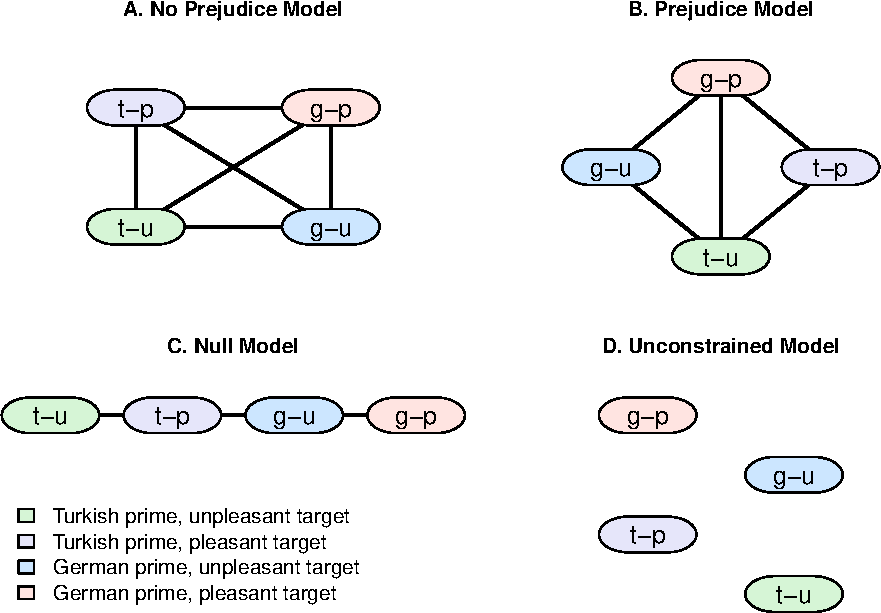
\includegraphics{p_files/figure-latex/anova-orders-1.pdf}
\caption{\label{fig:anova-orders}Theoretical positions are captured with order-constraints on cell means. Cells labeled \enquote{t-u} correspond to the condition with Turkish face prime and unpleasant target character, cells labeled \enquote{t-p} correspond to the condition with Turkish face prime and pleasant target character, cells labeled \enquote{g-u} correspond to the condition with German face prime and unpleasant target character, cells labeled \enquote{g-p} correspond to the condition with German face prime and pleasant target character. \textbf{A.} No-prejudice model were only target pleasantness has an effect on responses. \textbf{B.} Prejudice model were both target pleasantness and primes have an effect. \textbf{C.} Null model where there is no effect of target pleasantness and primes. \textbf{D.} None-of-the-above alternative model where all orderings of cell means are possible.}
\end{figure}

Multiple ordinal constraints arise naturally when several variables are manipulated factorially. These factorial designs are typically analyzed with an ANOVA. With this example we illustrate what ordinal constraints are and how the use of many of them simultaneously better capture relations between theory and data than does traditional ANOVA. Our example comes from a relatively new method for studying implicit attitudes, the affective misattribution procedure (AMP, Payne \& Lundberg, 2014). We highlight the study and results of Teige-Mocigemba, Becker, Sherman, Reichardt, and Klauer (2017) who investigated the possibility of using AMP as an implicit measure of prejudice.

In their task Teige-Mocigemba et al. (2017) briefly presented participants with prime stimuli that were chosen to elicit prejudicial attitudes.
These primes were pictures of Turkish and German faces. The study took place in Germany, and consequently, it is safe to presume that Turkish faces elicit more negative attitudes than German faces. After the prime was flashed, a Chinese character was presented, and participants were instructed to judge whether the character is pleasant or unpleasant. Unbeknownst to the participants, the particular Chinese characters were previously selected to be slightly pleasant or slightly unpleasant as determined by independent raters. There are two factors: the prime (Turkish vs.~German face) and the target pre-rated valence (previously rated pleasant character vs.~previously rated unpleasant character).

This target pleasantness manipulation is helpful from a pragmatic view for eliciting \emph{implicit} attitudes. Because the targets tend to have pre-established valences, the pleasantness task does not feel contrived. Importantly, participants believe they can focus on the characters pleasantness irrespective of the prime.

Though the target manipulation is helpful from a pragmatic view, it does not have a theoretical role. The key manipulation with a theoretical link to prejudice is the face prime manipulation, and the main question is whether there is an effect of this manipulation based on underlying prejudices towards Turkish people in the German population.
The theoretical prediction is therefore as follows: If prejudice affects the pleasantness ratings then pleasant targets are evaluated as pleasant more often when presented after a German face prime than when presented after a Turkish face prime. Likewise, unpleasant targets are evaluated as unpleasant more often when presented after a Turkish face prime than when presented after a German face prime.

There are two theoretical positions for this example:

\begin{itemize}
\item
  \emph{No-prejudice model}: Only target pleasantness affects the pleasantness decision in the AMP. There is no effect of the primes, i.e.~either the participants do not have prejudicial attitudes, or prejudicial attitudes do not affect the AMP. This position is shown graphically in Figure~\ref{fig:anova-orders}A. The four nodes represent the cell means in the design. The vertical and diagonal lines represent the relation of \enquote{more pleasant ratings than}, the horizontal lines represent the relation of \enquote{equally pleasant as}. The no-prejudice model predicts an equality of pleasantness ratings across prime conditions. Unpleasant targets remain equally unpleasant when preceded by Turkish and German faces; pleasant targets remain equally pleasant when preceded by Turkish and German faces.
\item
  \emph{Prejudice model}: In addition to target pleasantness there is an effect of prime ethnicity on the ratings. The position is shown in Figure~\ref{fig:anova-orders}B. Again, connections between nodes at different vertical levels represent \enquote{more pleasant ratings than} relations. Unconnected nodes have no relation regardless of their vertical position. The prediction from the prejudice model is that Turkish face primes followed by unpleasant targets have the lowest proportion of pleasant ratings. Accordingly, there are two paths to increase the target pleasantness ratings. One is to use more pleasant targets; the other is to precede the targets by German face primes. Note that there is no statement about which path is more effective---the prejudice model is agnostic to whether a German face prime of unpleasant targets leads to higher or lower ratings than a Turkish face prime of pleasant targets. The highest ratings are produced by pleasant targets preceded by German face primes.
\end{itemize}

One feature of psychological science is that there is not a one-to-one mapping from theories to potential data patterns. Some data patterns are simply not predicted by any theory under consideration. And yet such a pattern may occur. In our case, we know of no theoretical prediction for higher ratings of unpleasant targets than pleasant targets.
Likewise, neither the original authors nor us predicted that there would be no effect at all of the target manipulation.
We think it is wise to include a more constrained set of null models than the theoretically motivated models.
Figure~\ref{fig:anova-orders}C shows a \emph{null model} that predicts equal endorsements of pleasant responses in all conditions. The model captures the case that the pleasantness ratings are just not sensitive which is useful in interpreting a null prejudice effect. Indeed, if this model is preferred we would be more likely to worry about the overall sensitivity of the design than to conclude that there is not prejudice.
Likewise it is also wise to include models that are more general than the theoretically motivated models. Figure~\ref{fig:anova-orders}D shows an \emph{unconstrained model} where there are no relations.
All orderings of cells are possible. This model is preferred to any of the more constrained ones if none of the theories are doing a particularly good job at predicting the data.

\hypertarget{multiple-ordinal-constraints}{%
\subsection{Multiple Ordinal Constraints}\label{multiple-ordinal-constraints}}

Now we ready to give more formal meaning to multiple ordinal constraints. They are known, formally speaking, as \emph{partial weak orders}. They are \emph{weak} in that they may include equalities and they are \emph{partial} in that not all nodes have to be connected. Figure~\ref{fig:fig-hypothetical} further illustrates partial weak orders. Here there are six cells, and there is an ordering where Cell 1 is greater than Cells 2, 3, 4, 5, which in turn are greater than Cell 6.
There are equalities, Cells 2 and 3 are equal as are Cells 4 and 5. And there is partiality---no relations are defined between select cells such as Cells 2 and 4. Partial weak orders even include a lack of ordinal constraints, as shown in Figure~\ref{fig:fig-hypothetical}B. As can be seen these partial weak orders can capture a large variety of relations among cells. We use the phrase \emph{multiple ordinal constraints} as a less technical stand-in that emphasizes that there may be many equality and inequality statements that hold simultaneously.

\begin{figure}
\centering
\includegraphics{p_files/figure-latex/fig-hypothetical-1.pdf}
\caption{\label{fig:fig-hypothetical}Hypothetical systems of orders. \textbf{A.} Example of a partial weak order for six cells. \textbf{B.} A partial order may be unconstrained.}
\end{figure}

To implement multiple order constraints in this example, we start with a cornerstone parameterization (Rouder et al., 2016a). Let \(Y_{ijk}\) denote the proportion of pleasant responses for the \(i\)th participant in the \(j\)th prime condition (\(j=1, 2\), for Turkish face and German face primes, respectively), and in the \(k\)th target condition (\(k = 1, 2\) for unpleasant and pleasant targets, respectively). We define the anticipated least pleasant condition---unpleasant targets preceded by Turkish face primes---as the cornerstone condition. With this definition we model\footnote{Here, we demonstrate how cell means could be modeled with a linear model on proportions of binary outcomes. This approach is problematic because the proportions can only take on values between zero and one, but additivity in the linear model does not respect this range constraint. The simplification is used to ease the reader's burden. Alternatives are discussed in the Conclusions and Limitations section.} responses as

\[Y_{ijk} = \mu_i + x_{1} \alpha + x_{2} \beta + x_{3} \gamma + \epsilon_{ijk},\]

where \(\mu_i\) is each individuals' proportion of pleasant endorsements in the cornerstone condition. Parameter \(\alpha\) is the effect of the prime manipulation, parameter \(\beta\) is the effect of the target manipulation, and parameter \(\gamma\) is the over-additivity effect of the condition pleasant targets preceded by German face primes. Consequently, \(\gamma\) represents an interaction term. The indicator variables are \(x_1\) (0 for Turkish face primes and 1 for German face primes), \(x_2\) (0 for unpleasant targets and 1 for pleasant targets), and \(x_3\) (1 for pleasant targets preceded by German primes and 0 for all other combinations). Noise terms \(\epsilon_{ijk}\) are zero-centered and normally distributed.

The next step is to implement the four theory-driven models. In all the models \(\mu_i\) is unconstrained.

For the no-prejudice model, the parameters are constrained as follows:

\[
\begin{aligned}
\beta &>  0,\\
\alpha &= \gamma = 0.
\end{aligned}
\]

Here, \(\beta\), the effect of target pleasantness manipulation, is predicted to be positive so that target characters that were pre-rated as slightly positive elicit higher pleasantness ratings as target characters that were pre-rated as slightly negative. This effect is a key prediction from the affective misattribution procedure and does not correspond to any effects of prejudice. Parameter \(\alpha\), on the other hand, represents the effect of the face prime manipulation. For the no-prejudice model this case is instantiated by an equality constraint of \(\alpha = 0\). Likewise, in the absence of a prejudice effect there should not be an over-additive effect of target manipulation and face prime manipulation, resulting in the equality constraint that \(\gamma = 0\).

The prejudice model constrains the parameters as follows:

\[
\begin{aligned}
\alpha &>  0, \\ 
\beta &>  0, \\
\gamma &> -\alpha,\\
\gamma &> -\beta.
\end{aligned}
\]

The prejudice model is instantiated by four ordinal constraints. 1. The cell mean of the Turkish face prime and pleasant target condition has to be greater than the cell mean of the Turkish face prime and unpleasant target condition. This condition corresponds to the inequality constraint that \(\alpha > 0\). This constraint is the same as for the no-prejudice model. 2. The cell mean of the German face prime and unpleasant target condition has to be greater than the cell mean of the Turkish face prime and unpleasant target condition. This condition corresponds to the inequality constraint that \(\beta > 0\). 3. The cell mean of the German face prime and pleasant target condition (\(= \mu + \alpha + \beta + \gamma\)) has to be greater than the cell mean of the German face prime and unpleasant target condition (\(= \mu + \beta\)). To meet this condition, the inequality constraint \(\alpha + \gamma > 0\) has to hold, which is equivalent to \(\gamma > -\alpha\). 4. The cell mean of the German face prime and pleasant target condition (\(= \mu + \alpha + \beta + \gamma\)) has to be greater than the cell mean of the Turkish face prime and pleasant target condition (\(= \mu + \alpha\)). To meet this condition, the inequality constraint \(\beta + \gamma > 0\) has to hold, which is equivalent to \(\gamma > -\beta\).

The null model and the unconstrained model can also be expressed as constraints on \(\alpha\), \(\beta\), and \(\gamma\). The unconstrained model does not set any ordinal or equality constraints on these parameters; the null model has the following constraints:

\[\alpha = \beta = \gamma = 0,\]

indicating that the cell means for all four conditions have to be equal.

The models introduced here allows for better correspondence between theoretical claims and statistical models than does conventional ANOVA analysis. If these data were analyzed with ANOVA, the key tests would be whether the main effects of target pleasantness and face prime manipulations and their interaction are equal to zero or not. Note that this type of analysis cannot distinguish between the four above models. For example, both the prejudice model and the unconstrained model can predict an interaction between prime and target conditions (\(\gamma \neq 0\)).

\hypertarget{evaluating-multiple-ordinal-constraints}{%
\subsection{Evaluating Multiple Ordinal Constraints}\label{evaluating-multiple-ordinal-constraints}}

Encoding theories as multiple ordinal constraints raises a set of statistical considerations---how to assess evidence from data for competing sets of constraints. This assessment not only requires stating positive evidence for equality and inequality constraints, but doing so across many constraints simultaneously. Fortunately, Bayesian inference with Bayes factors is conceptually straightforward for assessing many equality and inequality constraints simultaneously (Gelfand, Smith, \& Lee, 1992; Jeffreys, 1961).

\begin{figure}
\centering
\includegraphics{p_files/figure-latex/comp-simple-1.pdf}
\caption{\label{fig:comp-simple}Model and predictions for one effect. \textbf{A.} The black arrow shows the prior for no effect, the blue curve shows the prior distribution for a positive effect, and the red curve shows the prior distribution for an unconstrained effect (i.e.~can be negative or positive). Higher values represent higher plausibility of the true effect before the data have been observed. \textbf{B.} The curves show predictions for observed effects for each prior. Predictions take into account sample noise and are smeared versions of the models themselves. The green vertical line represents a hypothetical observed effect. The data are best predicted by the positive-effect model compared to no-effect and unconstrained-effect.}
\end{figure}

How does Bayes factors model comparison work in practice for assessing evidence for ordinal constraints? We start with a very simple example first and then expand it to more complicated cases next. For the simple example, suppose we have data from a normal model as \(Y_i \sim \mbox{Normal}(\mu,\sigma^2)\). We have three positions: (i) a null constraint that \(\mu=0\); (ii) a positive constraint that \(\mu>0\); and (iii) an unconstrained position that \(mu\) can be any value (\(-\infty<\mu<\infty\)). Figure~\ref{fig:comp-simple}A shows models embedding these constraints. The spike at zero denotes the null constraint, that is all the mass for \(\mu\) is concentrated at zero. The positive curve shows a model that captures the positive constraint, and the curve on both positive and negative values shows the unconstrained position. It is important to note that these constraints are on \emph{true effects} without any sample noise. In practice, however, we observe effects with sample noise, and for these \emph{observed effects}, the constraint only has to hold approximately. Panel B of Figure~\ref{fig:comp-simple} shows the predictions from the models on observed effects after accounting for sample noise. Once the predictions are known, model comparison is simple. All we need to do is note where the data fall (Rouder, Haaf, \& Aust, 2018; Rouder et al., 2016b). The green line in Panel B denotes a hypothetical observed sample mean, \(\hat{\mu}\). As can be seen, this sample mean is best predicted by the positive-constraint model because it predicts positive effects (unlike the null model) and \emph{only} positive effects (unlike the unconstrained model).

\begin{figure}

{\centering \includegraphics[height=8in]{p_files/figure-latex/ex1Fig-1} 

}

\caption{Model (left) and predictions (right) for the combination of two parameters, here the effect of the priming condition and target condition. Darker areas represent higher plausibility of target and prime effects before the data are collected. Predictions take into account sampling noise. The hypothetical data point is best predicted by the Model B with a positive target effect and no prime effect.}\label{fig:ex1Fig}
\end{figure}

What happens if inequality and equality constraints are placed on several parameters simultaneously? Here, we may return to the priming example as the difference between the models is defined by the combination of three parameters. Three parameters is a lot to visualize, so for demonstration purposes here we focus on the effects of prime and target conditions, \(\alpha\) and \(\beta\). The left panel in Figure~\ref{fig:ex1Fig} shows four potential models on the two parameters. The first panel corresponds to our null model where both effects are zero; the second panel corresponds to the no-prejudice model where the prime effect is zero while the target effect is positive; the third panel corresponds to the prejudice model where both prime and target effects are greater than zero; and the last panel corresponds to the unconstrained model where both effects may be positive or negative. The right column of Figure~\ref{fig:ex1Fig} again shows the predictions on observed effects from the models. The red point is based on hypothetical data, and it shows a case where both effects are positive with the target condition effect being larger than the prime condition effect. This data point is best predicted by the no-prejudice model (second row) followed by the prejudice model (third row), the unconstrained model (last row) and finally the null model (first row).

The above examples show that Bayes factors are a measure of which models best predict the observed data. Though conceptually simple, gathering these predictions is often computationally difficult because they come from marginalizing or integrating the parameters. To address these computational difficulties, we take separate computational paths for equality and inequality constraints. For equality constraints, we follow a conventional \(g\)-prior approach introduced by Zellner and Siow (1980) and developed for factorial designs by Rouder, Morey, Speckman, and Province (2012). For inequality constraints, we follow the encompassing approach by Klugkist and Hoijtink and colleagues who instantiate order constraints on linear model parameters (Klugkist \& Hoijtink, 2007; Klugkist, Laudy, \& Hoijtink, 2005; Mulder, Klugkist, Schoot, Meeus, \& Hoijtink, 2009). The combination of both approaches was introduced by Haaf and Rouder (2017), and we have used this combination in our recent research (Haaf \& Rouder, 2019; Rouder et al., 2019a). Computational details are provided in the above referenced papers.

\hypertarget{results}{%
\subsection{Results}\label{results}}

We are now ready to apply the four models to Teige-Mocigemba et al.'s data set. Their set is of unusually high quality: First, task parameters were based on seven pilot studies. Second, the experiment itself was preregistered. Third, the data set is well powered. It is comprised of 216 participants providing a total of 31,104 observations. Further information on the design and materials are found in Teige-Mocigemba et al. (2017).

Cell means and conventional confidence intervals are shown in Figure~\ref{fig:fig-anova}. Pleasant targets are clearly rated as pleasant more often than unpleasant targets across both face prime levels. There seems to be a small observed effect of face prime where targets preceded by German faces are rated as pleasant more often than targets preceded by Turkish faces. The lowest proportion of pleasantness responses is observed in the condition with unpleasant targets preceded by Turkish face primes, followed by the condition with unpleasant targets preceded by German face primes, followed by the condition with pleasant targets preceded by Turkish face primes, and the highest proportion of pleasantness responses is observed in the condition with pleasant targets preceded by German face primes. This observed ordering of cells is most concordant with the prejudice model.

\begin{figure}
\centering
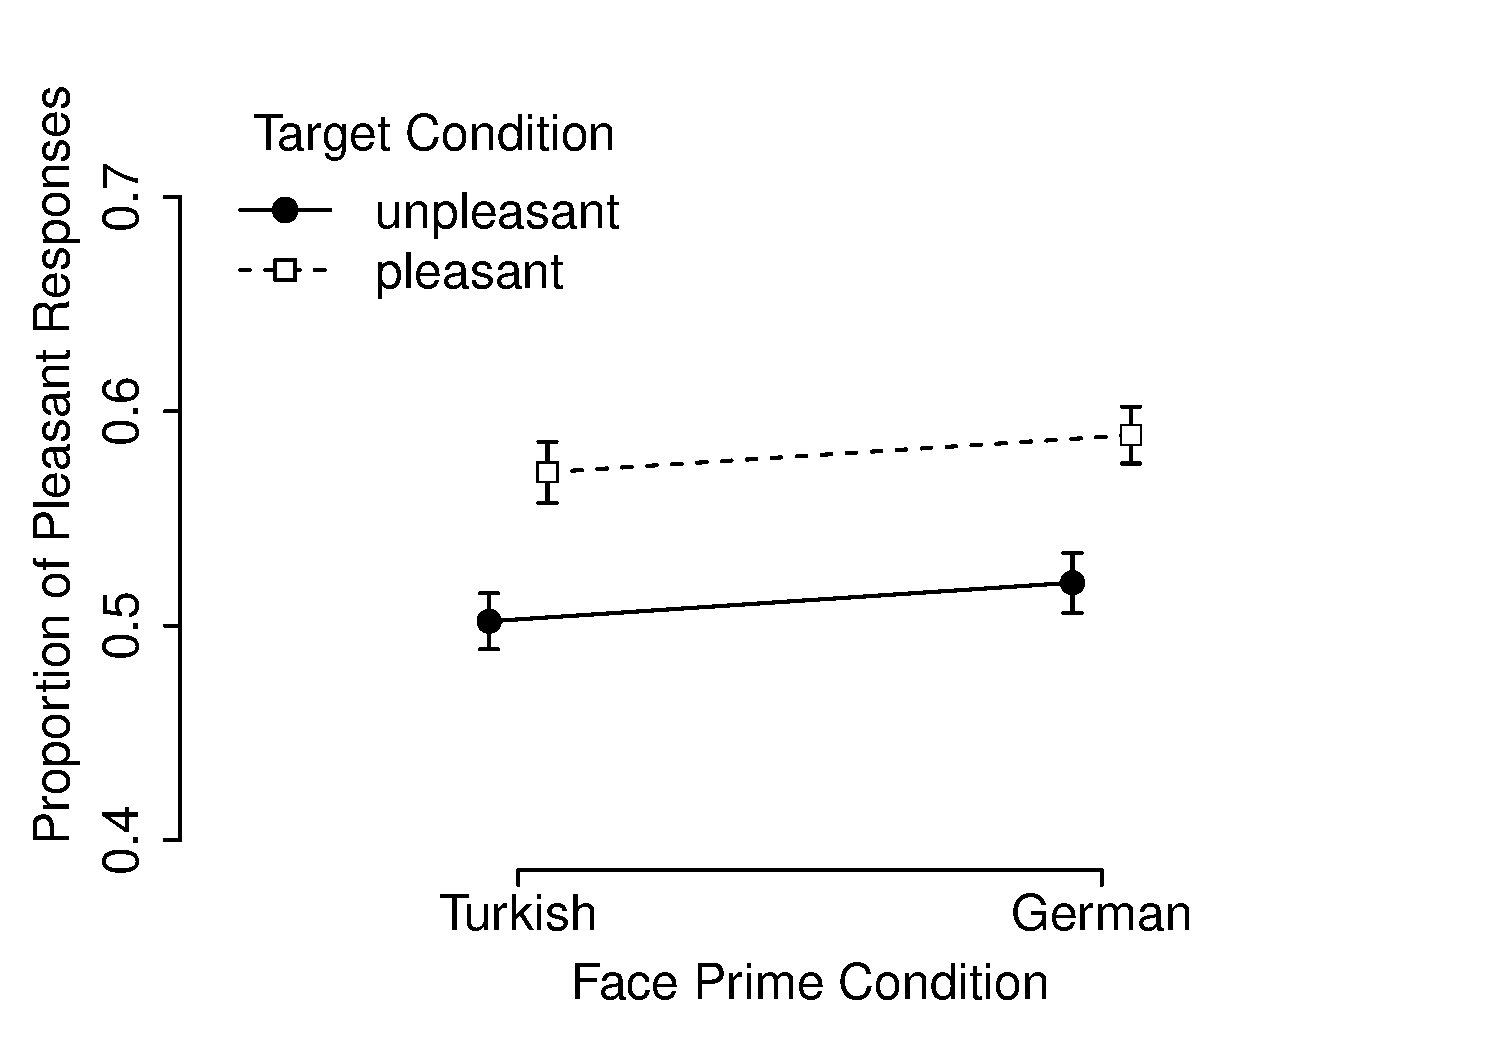
\includegraphics{p_files/figure-latex/fig-anova-1.pdf}
\caption{\label{fig:fig-anova}Prejudice data from Teige-Mocigemba et al.'s (2017) preregistered study. There is a clear effect of target condition in the expected direction and a small observed effect of prime condition in the expected direction.}
\end{figure}

Not surprisingly, in the model-based analysis the prejudice model is preferred over the other models with a Bayes factor of 4.40-to-one over the no-prejudice model, a Bayes factor of 5.43-to-one over the unconstrained model, and a Bayes factor of \(2.3 \times 10^{19}\)-to-one over the null model.

These results are somewhat in line with Teige-Mocigemba et al. (2017) who used a frequentist ANOVA and a subsequent posthoc test of the main effect of prime condition to analyse the prejudice effect. In a second analysis, the authors computed a directional Bayesian t-test on the main effect per person and found a Bayes factor of 2.8-to-one in favor of the prejudice effect. Here, we propose a more direct test of the target question by placing constraints on cell means and comparing different constraints in the Bayesian framework. With this direct approach we find more evidence for the position that there is an effect of prejudice in AMP than the original analysis. We do note that the degree of prejudice is small, which in itself is heartening.

\hypertarget{example-2-symbolic-distance}{%
\section{Example 2: Symbolic Distance}\label{example-2-symbolic-distance}}

In the above analysis we show how considering multiple ordinal constraints may provide for a more direct mapping between theory and inference than classical tests. Yet, in the previous example, the differences between conventional analysis and analysis by multiple ordinal constraints are relatively modest. In the following example we provide cases where the inference cannot be done in another way, and there is no analogous conventional analysis available.

The second example is based on a lexical effect from a task developed by Moyer and Landauer (1967). In this task the observer is presented with a digit, either 2, 3, 4, 6, 7, or 8, and has to decide whether the digit is greater than five or less than five. Participants are highly accurate, and the dependent variable of interest is the time to make the decision. The main question of interest is how does the time vary as a function of the digit, and in particular, does this time increase or decrease for digits further from five. Consider the following three theories:

\emph{Analog-Representation Theory} posits that numbers are stored in an analog system as a uni-dimensional quantity much like length (Gallistel \& Gelman, 1992). Just as comparing similar lengths is slower than disparate ones, this theory predicts that \(\mu_4>\mu_3>\mu_2\) and \(\mu_6>\mu_7>\mu_8\), where \(\mu_i\) is the true mean response time for the \(i\)th digit. This ordering is shown in Figure~\ref{fig:order}A.

\emph{Propositional Representation Theory} posits that numbers are represented as semantic propositions, much like in a computer. Accordingly, there should be no effect for distance-from-five. This theory leads to the equalities \(\mu_2=\mu_3=\mu_4\) and \(\mu_6=\mu_7=\mu_8\). We avoid specifying all six condition means are equal in case there is a speed difference across the \enquote{less than} and \enquote{greater than} responses. These equalities are represented in Figure~\ref{fig:order}B. Unconnected nodes have no relation; so even though the node \enquote{3} is above node \enquote{6}, there is no implied ordering because there is no line connecting the nodes.

\emph{Priming \(+\) Spreading Activation Theory} posits that familiar or anticipated items are responded to more quickly, that is, they are primed. Because participants need to keep the value of five in mind as part of the task demands, similar numbers are primed and responded to more quickly. Hence the semantic spreading activation network theory (Collins \& Loftus, 1975) predicts \(\mu_2>\mu_3>\mu_4\) and \(\mu_8>\mu_7>\mu_6\). This ordering is shown in Figure~\ref{fig:order}C; it is the reverse of that in Figure~\ref{fig:order}A.

\begin{figure}
\centering
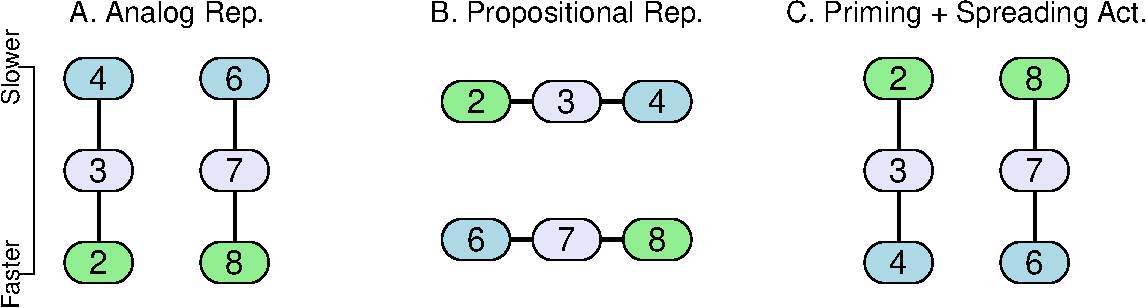
\includegraphics{p_files/figure-latex/order-1.pdf}
\caption{\label{fig:order}Depictions of orders for Examples 2 and 3. \textbf{A.} Analog representation in the symbolic distance task implies response times decrease with distance from five. \textbf{B.} Propositional representation implies no response time effects of distance. \textbf{C.} The priming account implies response times increase with distance from five.}
\end{figure}

In Moyer and Landauer (1967), response times tended to increase for digits close to 5. Consequently, Moyer \& Landauer concluded that number representation was analog. This finding remains influential in number cognition today.

\hypertarget{does-everybody}{%
\subsection{Does Everybody?}\label{does-everybody}}

In the preceding example, the focus is on the ordering of true population means, say whether the true mean response time for one condition is faster, slower, or the same as for another. For example, we might ask whether the orderings of population averages are more concordant with the analog-representation theory, the propositional-reasoning theory, or the spreading-activation theory. Yet, population averages are a fairly removed abstraction especially for the study of psychology.

A more insightful approach is to ask about individuals. Klaassen, Zedelius, Veling, Aarts, and Hoijtink (2017), focuses on assessing the correct set of ordinal constraints for each individual. Haaf and Rouder (2017) phrase the question a bit differently. Rather than focus on each individual's ordinal constraints, they ask whether all people obey the same ordinal constraints or whether there are individuals that obey different ordinal constraints. Haaf and Rouder (2017) call this the \emph{does everybody question.} In the context of the example, we may ask, does everybody follow the same theory, say analog representation, or are there differences. Perhaps it may be that while most people use analog representation, a minority uses propositional reasoning.

It is important to note that the focus is on true effects rather than sample scores. Even when the true effects of everybody in a population are in the same direction, we may observe some people who have scores that reverse the phenomenon-of-interest due to sample noise. The question then is, \emph{after accounting for sample noise, is it plausible that all individuals have true effects in the same direction, or, alternatively, is there evidence that some have true effects in the reverse direction.}

If all people show the same ordinal relations, we may consider this pattern to be lawful, automatic, perhaps biological, and perhaps largely outside of qualitative human variation. If not, say if some people have orders consistent with analog representation while others have orders consistent with propositional reasoning, we would examine theories with multiple representation systems.

\hypertarget{statistical-models-for-symbolic-distance}{%
\subsection{Statistical Models for Symbolic Distance}\label{statistical-models-for-symbolic-distance}}

Rouder, Lu, Speckman, Sun, and Jiang (2005) ran a standard symbolic distance experiment to assess how response times change with symbolic distance. Here, we consider the three systems of orders in Figure~\ref{fig:order}A-C: The Analog-Representation theory, the Propositional-Representation theory, and the Priming \(+\) Spreading-Activation theory. Moreover, we consider whether all participants have the same ordering. Let \(Y_{ijk}\) denote the response time for the \(i\)th participant in the \(j\)th digit condition (\(j=2, 3, 4, 6, 7, 8\)), and for the \(k\)th replicate:
\[Y_{ijk}|\nu_{ij},\sigma^2 \stackrel{ind}{\sim}\mbox{Normal}(\nu_{ij},\sigma^2),\]

where \(\nu_{ij}\) is the \(i\)th person's true mean response time for the \(j\)th condition, and \(\sigma^2\) is the trial-by-trial variation.
To represent the theories it is useful to reparameterize the above model into relative differences between condition means for each individual. The following appears complicated, but it is just a matter of defining the relevant contrasts within a linear model using dummy variables. Let \(\delta_{im}\) be the \(m\)th relative difference for the \(i\)th person. There are four of these relative differences implied by the theories defined as follows: \(\delta_{i1}=\nu_{i3}-\nu_{i2}\), \(\delta_{i2}=\nu_{i4}-\nu_{i3}\), \(\delta_{i3}=\nu_{i6}-\nu_{i7}\), and \(\delta_{i4}=\nu_{i7}-\nu_{i8}\). With these differences, the cell means \(\nu_{ij}\) are given as
\begin{equation}\label{modelex2}
\nu_{ij} = {s_j}\left(\nu_{i3} - x_{2j}\delta_{i1} + x_{4j}\delta_{i2}\right) + (1-s_j)\left(\nu_{i7} - x_{8j}\delta_{i4} + x_{6j}\delta_{i3}\right),
\end{equation}
where \(s_j=1\) for the digit conditions \(j<5\), and \(s_j=0\) for digit conditions \(j>5\); and \(x_{j'j}=1\) if the index \(j'\) indicates the current digit condition, \(j\). For example, for digit condition \(j = 2\) and participant \(i = 1\), \(s_j = 1\), \(x_{2j} = 1\), and \(x_{4j} = 0\). Therefore, \(\nu_{12} = \nu_{13} + \delta_{11}\).

With this reparameterization models may be placed on the relative differences, \(\delta_{im}\). These differences are defined so that they are a subtraction of a digit further from 5 from a digit that is closer to 5. Hence, positive values of \(\delta_{im}\) are consistent with the Analog-Representation theory where response times are larger for digits closer to 5.

\begin{figure}
\centering
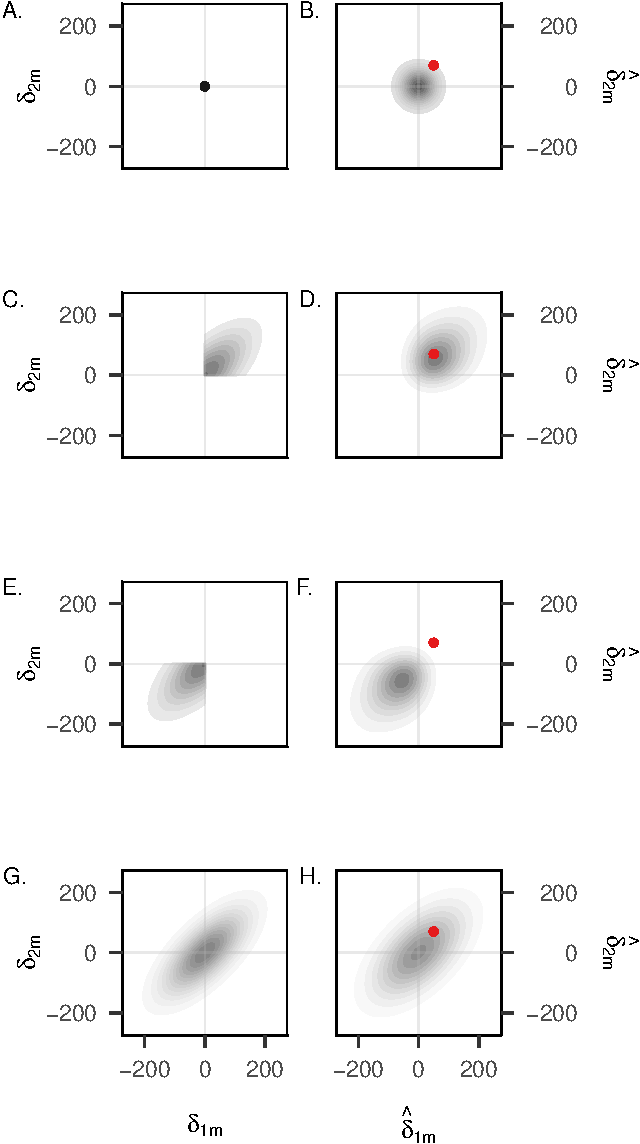
\includegraphics{p_files/figure-latex/modelplot-1.pdf}
\caption{\label{fig:modelplot}Models (left) and predictions (right) for the symbolic distance effect. Darker areas represent higher plausibility of \(\delta_{im}\) before the data are collected. Models are conditional on set values of \(\mu_m=0\)ms and \(\eta=90\)ms. Predictions take into account sampling noise and the correlation reflects the priors placed on \(\mu_m\) and \(\eta^2\). The red point represents a hypothetical observed data point for two individuals. The hypothetical data point is best predicted by the Analog-Representaion model.}
\end{figure}

The theories then correspond to the following constraints: 1. The Analog-Representation theory holds for the \(i\)th individual if \(\delta_{im}>0\) for each \(m\). 2. The Priming \(+\) Spreading-Activation theory holds for the \(i\)th individual if \(\delta_{im}<0\) for each \(m\). 3. The propositional-representation model holds for the \(i\)th individual if \(\delta_{im}=0\) for each \(m\).

In the next step, we write these constraints as formalized models on the collection of individuals' relative differences. Model \({\cal M}_0\) instantiates the statement that everybody uses propositional representation. It is given by
\[
{\cal M}_0: \quad \delta_{im}=0.
\]

Figure~\ref{fig:modelplot}A shows a graphical depiction of the propositional-representation model for two participants. The \(x\)-axis shows the true effect for one participant for the \(m\)th difference, \(\delta_{1m}\); the \(y\)-axis shows the true effect for a second participant, \(\delta_{2m}\). The only point with mass is \((0,0)\) showing that each participants' relative differences between digit conditions must be identically zero.

Model \({\cal M}_+\) instantiates the statement that everybody uses analog representation, and it is given by:
\[
{\cal M}_+: \quad \delta_{im}|\mu_m,\eta^2 \sim \mbox{Normal}_+(\mu_m,\eta^2),
\]

where Normal\(_+\) is a normal distribution truncated from below at zero, \(\mu_m\) is the population mean of the \(m\)th digit condition difference, and \(\eta^2\) is the variability of individuals around this mean. Figure~\ref{fig:modelplot}C depicts this model for two participants (for set values of \(\mu_m\) and \(\eta^2\)). For both participants, only positive values have mass.

Model \({\cal M}_-\) instantiates the statement that everybody uses priming \(+\) spreading activation, and it is given by:
\[
{\cal M}_-: \quad \delta_{im}|\mu_m,\eta^2 \sim \mbox{Normal}_-(\mu_m,\eta^2),
\]
where Normal\(_-\) is a normal truncated from above at zero. Figure~\ref{fig:modelplot}E depicts this model for two participants. For both participants only negative values have mass.

Of course, it may be that not everyone uses the same number representation system. We therefore implement a \enquote{none-of-the-above} model by placing no ordinal constraints on the relative differences. This model is termed the unconstrained model and is denoted \({\cal M}_u\):

\[
{\cal M}_u: \quad \delta_{im}|\mu_m,\eta^2 \sim \mbox{Normal}(\mu_m,\eta^2).
\]

If this model is strongly preferred, the interpretation is that none of the everybody-does models are appropriate. Consequently, we may conclude different people use different representations. Figure~\ref{fig:modelplot}G illustrates this model for two participants. Here, the participants' effects are not constrained to any of the quadrants.

Prior specifications are needed for \(\sigma^2\), \(\mu_m\), \(\eta^2\), \(\nu_3\) and \(\nu_7\). We take a \(g\)-prior approach as discussed in Haaf and Rouder (2017), and the prior specifications for this application are provided in the Appendix.

In Figure~\ref{fig:modelplot}, we show the model specification for any two participants on any one difference contrast (for any one value of \(m\)). For the symbolic-distance experiment by Rouder et al. (2005), however, four difference contrasts are specified, and 52 individuals participated in the experiment. The figure therefore understates the dramatic differences in constraint between the models. The constraints provided by the models must hold across all people and across all difference contrasts simultaneously.

\hypertarget{evaluating-multiple-constraints-in-hierarchical-models}{%
\subsection{Evaluating Multiple Constraints in Hierarchical Models}\label{evaluating-multiple-constraints-in-hierarchical-models}}

For the symbolic data we again use Bayes factors to evaluate the relative predictive accuracy of the models. The right column of Figure~\ref{fig:modelplot} shows the predictions on observed relative differences for the four models applied here. One aspect of these predictions that is not obvious is the correlation across participants. This correlation comes from the hierarchical structure in these models, and is a direct result of variability of the population mean, \(\mu_m\), as compared to the between-person variability, \(\eta^2\). This correlation across participants reduces the dimensionality of the model space, and this reduction eases the Bayes factor computations. Conceptually, once the correlations from the hierarchical structure are taken into account, model comparison again is simply a matter of observing where the data fall (i.e.~the red point in the figure) and to compare how well each model predicted the data. In Figure~\ref{fig:modelplot} the analog-representation model, \({\cal M}_+\), predicts the data best. A formal discussion of both the Bayes factor computations and the hierarchical structure of the models is provided in Haaf and Rouder (2017).

\hypertarget{results-1}{%
\subsection{Results}\label{results-1}}

\begin{figure*}
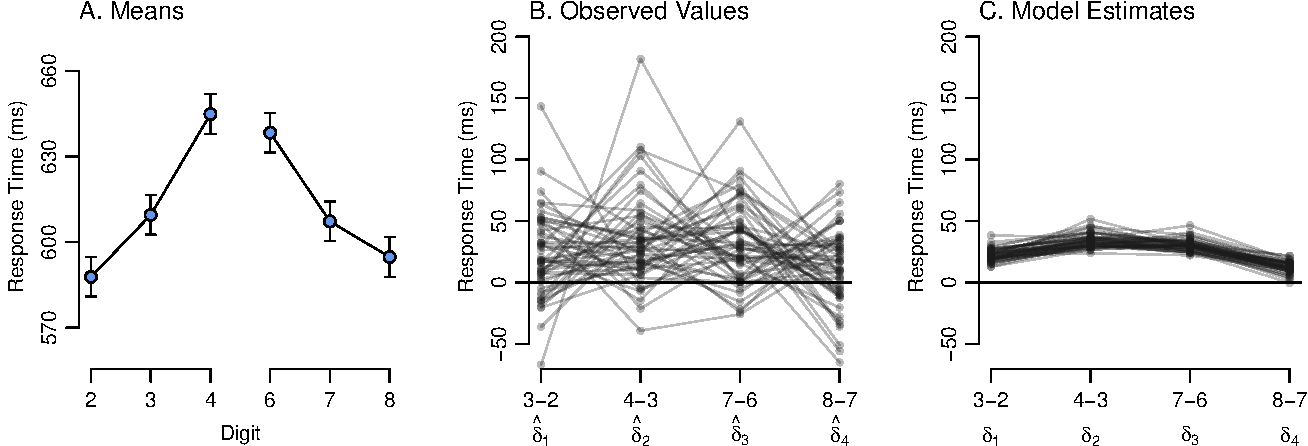
\includegraphics{p_files/figure-latex/ld5-1} \caption{Symbolic Distance effects: \textbf{A.} Condition means show a pattern indicative of analog representation.  \textbf{B.} Observed successive differences for all individuals.  Positive values are indicative of analog representation. \textbf{C.} Model estimates of successive differences from the unconstrained model.  There is much shrinkage indicating that much of the noise in the observed values is due to trial-by-trial noise.}\label{fig:ld5}
\end{figure*}

The results of the analysis of Rouder et al.'s (2005) data are shown in Figure~\ref{fig:ld5}. Panel A depicts sample means across people as a function of digit condition, and it is obvious that, at an aggregated level, the analog-representation explanation is preferred. The next question is whether all participants use this analog representation. Panel B shows the reparameterized participant-specific sample effects, \(\hat{\delta}_{im}\) for all people and differences. Recall that positive effects correspond to the analog-representation theory, negative effects correspond to the Priming \(+\) Spreading-Activation theory, and effects around zero correspond to the Propositional-Representation theory. As can be seen, there is a lot of variability. Even though the majority of individual effects are above zero, there is a large degree of variability. The variability in this example shows how difficult it is to answer the question of whether everybody uses an analog representation by inspecting sample effects. A model-based analysis is needed.

Panel C shows model-based estimates from the unconstrained model. Here, the hierarchical structure in the prior results in the regularization of effects. This degree of regularization implies that much of the variability in the sample means in Panel B reflects trial-to-trial noise. This type of regularization shows a key practical value of hierarchical models in analysis (Efron \& Morris, 1977; Gelman \& Carlin, 2017; Rouder et al., 2005). By inspection, all but one of the estimates are above zero. As a consequence, it may be tempting to use these estimates as evidence for the everybody-has-analog-representation constraint. Yet, more caution is needed. The individual estimates provided by the unconstrained model are not independent across persons, and as a consequence, observing which are above and below zero may be deceiving. For these data, estimation is useful for visualization, but it does not address the question of interest.

This question may be answered by computing Bayes factors for the four models. First, we compare the three \emph{everybody does} models. The clear winner is the analog-representation model, and it beats the propositional-representation model by over \(10^{55}\)-to-1. The priming \(+\) spreading-activation model performs so poorly that its decrement is outside of our numerical precision, and it is at least 100 orders worse than the analog-representation model. Second, we may also compare the analog-representation model to the unconstrained model, and the Bayes factor is 9.78-to-1 in favor of the former. The data provides therefore provides support for everybody-has-analog-representation as compared to the unconstrained model.

\hypertarget{conclusions-and-limitations}{%
\section{Conclusions and Limitations}\label{conclusions-and-limitations}}

Given the coarse state of theory in the social sciences, finding paths to improve testable constraint is timely and topical. One profitable avenue for increasing constraint is to propose multiple ordinal constraints simultaneously. Here, we develop principled and straightforward Bayesian inference that is broadly applicable to questions such as, \emph{is A greater than B}, \emph{is A less than B}, or \emph{is A equal to B}, and scales up well to questions such as \emph{does everyone,} \emph{do some}, or **do none.* It is our hope that these tools will motivate researchers to explicitly specify theory as multiple ordinal constraints.

There are perhaps three limitations of the current approach: 1. the use of parametric models, 2. the need for prior specifications, and 3. the lack of implementation of these methods in popular software platforms. We take these limitations in turn.

The current modeling approach is to place ordinal constraints on mean parameters in linear models with normally-distributed noise (Klugkist et al., 2005). One may wonder about the sensitivity of inference to the normal specification. In linear models, effects are assumed to shift the noise distribution without changing its scale or shape. The general consensus is that these specifications are not too problematic in classical inference (Hays, 1994). In our experience, both from simulation and in practice, Bayesian inference is robust to these parametric specifications (Haaf \& Rouder, 2019; Rouder et al., 2019a; Thiele, Haaf, \& Rouder, 2017). The reason is straight-forward---the effects we explore are so small relative to trial noise that the shifted normal is a fine approximation. Even for the mean proportions in the prejudice example we are comfortable that not too much damage is done by applying normal-noise models. For other types of data, alternatives to the parametric models are available (Heck \& Davis-Stober, 2019; Klaassen et al., 2017).

The more concerning limitation is the need to specify prior distributions with tuning settings. The main parameters of concern are those that differentiate the models. In the AMP example, these are the priors on \(\alpha\), \(\beta\), and \(\gamma\) as described in the Appendix. In the symbolic distance example, these are the priors on \(\mu_m\) and \(\eta^2\), also described in the Appendix. These priors define \emph{a priori} expectations about the overall effect and about between-person variability. The choice of these tuning parameters is a substantive choice rather than a statistical one, and researchers who are substantive experts in their domain should be unafraid to add value here. In the AMP example, we opted for weakly-informative priors based on the expectation that effects on implicit measures such as the AMP are usually small, and the interactions between them (i.e.~the \(\gamma\) parameter) tend to be even smaller. The prior settings in the symbolic distance example are also motivated from substantive knowledge: We reasoned that any distance-from-five effect is roughly on the order of 50 ms and between-person variability is roughly on the order of 30 ms. This is not to say that \(\mu_m\) and \(\eta^2\) are these values, but they come from distributions that reflect these settings. Our advise is that researchers should use a range of scale settings they find reasonable and track how inference changes across these settings. Detailed discussion and examples of this approach may be found in Rouder et al. (2016b) and Haaf and Rouder (2017).

The final limitation is that the current analyses are not yet available in popular packages. Perhaps the easiest software package for computing Bayes factors is \texttt{JASP} (Love et al., 2015). This package was reverse engineered to look and feel like \texttt{SPSS}, and users familiar with with \texttt{SPSS} can use \texttt{JASP} easily. \texttt{JASP} has some options to evaluate inequality constraints implemented, but is not yet set up to analyze systems of order constraints more generally. Alternatively, there are several \texttt{R} packages that allow for model comparison with ordinal constraints using Bayes factors. Examples are \texttt{BAIN} (Gu, Mulder, \& Hoijtink, n.d.) and \texttt{BayesFactor} (Morey \& Rouder, 2015) that both allow for the evaluation of equality and inequality constraints. Yet, using these packages for the implementation of constraints on individuals' effects in hierarchical settings is more involved. The source code for this paper is an example of this adaptation using \texttt{BayesFactor} (see \href{https://github.com/PerceptionAndCognitionLab/bf-order/tree/public/papers/submission}{here}). While the current software situation is fluid and there are turn-key solutions for only a handful of models, we suspect that easy-to-use packages addressing a full range of order constraints will be available soon.

\hypertarget{open-practices-statement}{%
\section{Open Practices Statement}\label{open-practices-statement}}

The authors advocate for and adhere to a fully transparent research pipeline (Rouder et al., 2019b). This transparency includes making data and analysis code openly accessible.

\begin{itemize}
\item
  The data analyzed here were previously collected by Teige-Mocigemba et al. (2017) (Example 1) and Rouder et al. (2005) (Example 2). Both datasets are publicly available on github.com (\href{https://osf.io/vcz4a/}{Example 1} and \href{https://raw.githubusercontent.com/PerceptionCognitionLab/data0/master/lexDec-dist5/ld5.all}{Example 2}).
\item
  The document for this paper, with all text and code, can be found at \url{https://github.com/PerceptionAndCognitionLab/bf-order/tree/public/papers/submission}.
\end{itemize}

Please contact the first author in case there are any questions about the data or analysis.

\newpage

\hypertarget{references}{%
\section{References}\label{references}}

\begingroup
\setlength{\parindent}{-0.5in}
\setlength{\leftskip}{0.5in}

\hypertarget{refs}{}
\leavevmode\hypertarget{ref-Cohen:etal:1990}{}%
Cohen, J., Dunbar, K., \& McClelland, J. (1990). On the control of automatic processes: A parallel distributed processing account of the stroop effect. \emph{Psychological Review}, \emph{97}, 332--361.

\leavevmode\hypertarget{ref-Collins:Loftus:1975}{}%
Collins, A., \& Loftus, E. (1975). A spreading-activation theory of semantic processing. \emph{Psychological Review}, \emph{82}, 407--428.

\leavevmode\hypertarget{ref-Efron:Morris:1977}{}%
Efron, B., \& Morris, C. (1977). Stein's paradox in statistics. \emph{Scientific American}, \emph{236}, 119--127.

\leavevmode\hypertarget{ref-Gallistel:Gelman:1992}{}%
Gallistel, C. R., \& Gelman, R. (1992). Preverbal and verbal counting and computation. \emph{Cognition}, \emph{44}, 43--74.

\leavevmode\hypertarget{ref-Gelfand:etal:1992}{}%
Gelfand, A. E., Smith, A. F. M., \& Lee, T.-M. (1992). Bayesian analysis of constrained parameter and truncated data problems using Gibbs sampling. \emph{Journal of the American Statistical Association}, \emph{87}(418), 523--532. Retrieved from \url{http://www.jstor.org/stable/2290286}

\leavevmode\hypertarget{ref-Gelman:Carlin:2017}{}%
Gelman, A., \& Carlin, J. (2017). \emph{Some natural solutions to the \(p\)-value communication problem---and why they won't work}.

\leavevmode\hypertarget{ref-Gelman:etal:2004}{}%
Gelman, A., Carlin, J. B., Stern, H. S., \& Rubin, D. B. (2004). \emph{Bayesian data analysis (2nd edition)}. London: Chapman; Hall.

\leavevmode\hypertarget{ref-Gu:etal:inpress}{}%
Gu, X., Mulder, J., \& Hoijtink, H. (n.d.). Approximated adjusted fractional bayes factors: A general method for testing informative hypotheses. \emph{British Journal of Mathematical and Statistical Psychology}. Retrieved from \url{http://dx.doi.org/10.1111/bmsp.12110}

\leavevmode\hypertarget{ref-Haaf:Rouder:2017}{}%
Haaf, J. M., \& Rouder, J. N. (2017). Developing constraint in Bayesian mixed models. \emph{Psychological Methods}, \emph{22}(4), 779--798.

\leavevmode\hypertarget{ref-Haaf:Rouder:2019}{}%
Haaf, J. M., \& Rouder, J. N. (2019). Some do and some don't? Accounting for variability of individual difference structures. \emph{Psychonomic Bulletin and Review}. Retrieved from \url{https://psyarxiv.com/zwjtp/}

\leavevmode\hypertarget{ref-Hays:1994}{}%
Hays, W. L. (1994). \emph{Statistics} (fifth.). Ft. Worth, T.X.: Harcourt Brace.

\leavevmode\hypertarget{ref-Heck:Davis-Stober:2019}{}%
Heck, D. W., \& Davis-Stober, C. P. (2019). Multinomial models with linear inequality constraints: Overview and improvements of computational methods for bayesian inference. \emph{Journal of Mathematical Psychology}, \emph{91}, 70--87.

\leavevmode\hypertarget{ref-Jeffreys:1961}{}%
Jeffreys, H. (1961). \emph{Theory of probability (3rd edition)}. New York: Oxford University Press.

\leavevmode\hypertarget{ref-Kahneman:1973}{}%
Kahneman, D. (1973). \emph{Attention and effort}. Englewood Cliffs, NJ: Prentice-Hall.

\leavevmode\hypertarget{ref-Klaassen:etal:2017}{}%
Klaassen, F., Zedelius, C., Veling, H., Aarts, H., \& Hoijtink, H. (2017). All for one or some for all? Evaluating informative hypotheses for multiple N=1 studies. \emph{Behavior Research Methods}. Retrieved from \url{10.3758/s13428-017-0992-5}

\leavevmode\hypertarget{ref-Klugkist:Hoijtink:2007}{}%
Klugkist, I., \& Hoijtink, H. (2007). The Bayes factor for inequality and about equality constrained models. \emph{Computational Statistics \& Data Analysis}, \emph{51}(12), 6367--6379.

\leavevmode\hypertarget{ref-Klugkist:etal:2005}{}%
Klugkist, I., Laudy, O., \& Hoijtink, H. (2005). Inequality constrained analysis of variance: A bayesian approach. \emph{Psychological Methods}, \emph{10}(4), 477.

\leavevmode\hypertarget{ref-Lee:Wagenmakers:2013}{}%
Lee, M. D., \& Wagenmakers, E.-J. (2013). \emph{Bayesian cognitive modeling: A practical course}. Cambridge University Press.

\leavevmode\hypertarget{ref-Lewandowsky:Farrell:2011}{}%
Lewandowsky, S., \& Farrell, S. (2011). \emph{Computational modeling in cognition: Principles and practice}. Thousand Oaks, CA: Sage.

\leavevmode\hypertarget{ref-Logan:1988}{}%
Logan, G. D. (1988). Towards an instance theory of automization. \emph{Psychological Review}, \emph{95}, 492--527.

\leavevmode\hypertarget{ref-Love:etal:2015}{}%
Love, J., Selker, R., Verhagen, J., Smira, M., Wild, A., Marsman, M., \ldots{} Wagenmakers, E.-J. (2015). Software to sharpen your stats. \emph{APS Observer}, \emph{28}, 27--29.

\leavevmode\hypertarget{ref-Morey:Rouder:BayesFactorPackage}{}%
Morey, R. D., \& Rouder, J. N. (2015). BayesFactor 0.9.12-2. Comprehensive R Archive Network. Retrieved from \url{http://cran.r-project.org/web/packages/BayesFactor/index.html}

\leavevmode\hypertarget{ref-Moyer:Landauer:1967}{}%
Moyer, R. S., \& Landauer, T. K. (1967). Time required for judgements of numerical inequality. \emph{Nature}, \emph{215}, 1519--1520.

\leavevmode\hypertarget{ref-Mulder:etal:2009}{}%
Mulder, J., Klugkist, I., Schoot, R. van de, Meeus, W. H. J., \& Hoijtink, H. (2009). Bayesian model selection of informative hypotheses for repeated measurements. \emph{Journal of Mathematical Psychology}, \emph{54}(530-546).

\leavevmode\hypertarget{ref-Payne:Lundberg:2014}{}%
Payne, K., \& Lundberg, K. (2014). The affect misattribution procedure: Ten years of evidence on reliability, validity, and mechanisms. \emph{Social and Personality Psychology Compass}, \emph{8}(12), 672--686.

\leavevmode\hypertarget{ref-Rouder:etal:2016d}{}%
Rouder, J. N., Engelhardt, C. R., McCabe, S., \& Morey, R. D. (2016a). Model comparison in anova. \emph{Psychonomic Bulletin \& Review}, \emph{23}(6), 1779--1786. Retrieved from \url{https://doi.org/10.3758/s13423-016-1026-5}

\leavevmode\hypertarget{ref-Rouder:etal:2018}{}%
Rouder, J. N., Haaf, J. M., \& Aust, F. (2018). From theories to models to predictions: A Bayesian model comparison approach. \emph{Communication Monographs}, \emph{85}, 41--56. Retrieved from \url{https://doi.org/10.1080/03637751.2017.1394581}

\leavevmode\hypertarget{ref-Rouder:etal:2019b}{}%
Rouder, J. N., Haaf, J. M., Davis-Stober, C. P., \& Hilgard, J. (2019a). Beyond overall effects: A Bayesian approach to finding constraints in meta-analysis. \emph{Psychological Methods}.

\leavevmode\hypertarget{ref-Rouder:etal:2019a}{}%
Rouder, J. N., Haaf, J. M., \& Snyder, H. K. (2019b). Minimizing mistakes in psychological science. \emph{Advances in Methods and Practices in Psychological Science}.

\leavevmode\hypertarget{ref-Rouder:etal:2005a}{}%
Rouder, J. N., Lu, J., Speckman, P. L., Sun, D., \& Jiang, Y. (2005). A hierarchical model for estimating response time distributions. \emph{Psychonomic Bulletin and Review}, \emph{12}, 195--223.

\leavevmode\hypertarget{ref-Rouder:etal:2012}{}%
Rouder, J. N., Morey, R. D., Speckman, P. L., \& Province, J. M. (2012). Default Bayes factors for ANOVA designs. \emph{Journal of Mathematical Psychology}, \emph{56}, 356--374. Retrieved from \url{http://dx.doi.org/10.1016/j.jmp.2012.08.001}

\leavevmode\hypertarget{ref-Rouder:etal:2016b}{}%
Rouder, J. N., Morey, R. D., \& Wagenmakers, E.-J. (2016b). The interplay between subjectivity, statistical practice, and psychological science. \emph{Collabra}, \emph{2}, 6. Retrieved from \url{http://doi.org/10.1525/collabra.28}

\leavevmode\hypertarget{ref-Smith:2000}{}%
Smith, P. L. (2000). Stochastic dynamic models of response time and accuracy: A foundational primer. \emph{Journal of Mathematical Psychology}, \emph{44}, 408--463.

\leavevmode\hypertarget{ref-Stroop:1935}{}%
Stroop, J. R. (1935). Studies of interference in serial verbal reactions. \emph{Journal of Experimental Psychology}, \emph{18}, 643--662.

\leavevmode\hypertarget{ref-Teige-Mocigemba:etal:2017}{}%
Teige-Mocigemba, S., Becker, M., Sherman, J. W., Reichardt, R., \& Klauer, K. C. (2017). The affect misattribution procedure. \emph{Experimental Psychology}, \emph{64}(3). Retrieved from \url{10.1027/1618-3169/a000364}

\leavevmode\hypertarget{ref-Thiele:etal:2017}{}%
Thiele, J. E., Haaf, J. M., \& Rouder, J. N. (2017). Bayesian analysis for systems factorial technology. \emph{Journal of Mathematical Psychology}, \emph{81}, 40--54.

\leavevmode\hypertarget{ref-Townsend:Ashby:1983}{}%
Townsend, J. T., \& Ashby, F. G. (1983). \emph{Stochastic modeling of elementary psychological processes}. London: Cambridge.

\leavevmode\hypertarget{ref-Zellner:1986}{}%
Zellner, A. (1986). On assessing prior distirbutions and Bayesian regression analysis with \(g\)-prior distribution. In P. K. Goel \& A. Zellner (Eds.), \emph{Bayesian inference and decision techniques: Essays in honour of Bruno de Finetti} (pp. 233--243). Amsterdam: North Holland.

\leavevmode\hypertarget{ref-Zellner:Siow:1980}{}%
Zellner, A., \& Siow, A. (1980). Posterior odds ratios for selected regression hypotheses. In J. M. Bernardo, M. H. DeGroot, D. V. Lindley, \& A. F. M. Smith (Eds.), \emph{Bayesian statistics: Proceedings of the First International Meeting held in Valencia (Spain)} (pp. 585--603). University of Valencia.

\leavevmode\hypertarget{ref-Cohen:etal:1990}{}%
Cohen, J., Dunbar, K., \& McClelland, J. (1990). On the control of automatic processes: A parallel distributed processing account of the stroop effect. \emph{Psychological Review}, \emph{97}, 332--361.

\leavevmode\hypertarget{ref-Collins:Loftus:1975}{}%
Collins, A., \& Loftus, E. (1975). A spreading-activation theory of semantic processing. \emph{Psychological Review}, \emph{82}, 407--428.

\leavevmode\hypertarget{ref-Efron:Morris:1977}{}%
Efron, B., \& Morris, C. (1977). Stein's paradox in statistics. \emph{Scientific American}, \emph{236}, 119--127.

\leavevmode\hypertarget{ref-Gallistel:Gelman:1992}{}%
Gallistel, C. R., \& Gelman, R. (1992). Preverbal and verbal counting and computation. \emph{Cognition}, \emph{44}, 43--74.

\leavevmode\hypertarget{ref-Gelfand:etal:1992}{}%
Gelfand, A. E., Smith, A. F. M., \& Lee, T.-M. (1992). Bayesian analysis of constrained parameter and truncated data problems using Gibbs sampling. \emph{Journal of the American Statistical Association}, \emph{87}(418), 523--532. Retrieved from \url{http://www.jstor.org/stable/2290286}

\leavevmode\hypertarget{ref-Gelman:Carlin:2017}{}%
Gelman, A., \& Carlin, J. (2017). \emph{Some natural solutions to the \(p\)-value communication problem---and why they won't work}.

\leavevmode\hypertarget{ref-Gelman:etal:2004}{}%
Gelman, A., Carlin, J. B., Stern, H. S., \& Rubin, D. B. (2004). \emph{Bayesian data analysis (2nd edition)}. London: Chapman; Hall.

\leavevmode\hypertarget{ref-Gu:etal:inpress}{}%
Gu, X., Mulder, J., \& Hoijtink, H. (n.d.). Approximated adjusted fractional bayes factors: A general method for testing informative hypotheses. \emph{British Journal of Mathematical and Statistical Psychology}. Retrieved from \url{http://dx.doi.org/10.1111/bmsp.12110}

\leavevmode\hypertarget{ref-Haaf:Rouder:2017}{}%
Haaf, J. M., \& Rouder, J. N. (2017). Developing constraint in Bayesian mixed models. \emph{Psychological Methods}, \emph{22}(4), 779--798.

\leavevmode\hypertarget{ref-Haaf:Rouder:2019}{}%
Haaf, J. M., \& Rouder, J. N. (2019). Some do and some don't? Accounting for variability of individual difference structures. \emph{Psychonomic Bulletin and Review}. Retrieved from \url{https://psyarxiv.com/zwjtp/}

\leavevmode\hypertarget{ref-Hays:1994}{}%
Hays, W. L. (1994). \emph{Statistics} (fifth.). Ft. Worth, T.X.: Harcourt Brace.

\leavevmode\hypertarget{ref-Heck:Davis-Stober:2019}{}%
Heck, D. W., \& Davis-Stober, C. P. (2019). Multinomial models with linear inequality constraints: Overview and improvements of computational methods for bayesian inference. \emph{Journal of Mathematical Psychology}, \emph{91}, 70--87.

\leavevmode\hypertarget{ref-Jeffreys:1961}{}%
Jeffreys, H. (1961). \emph{Theory of probability (3rd edition)}. New York: Oxford University Press.

\leavevmode\hypertarget{ref-Kahneman:1973}{}%
Kahneman, D. (1973). \emph{Attention and effort}. Englewood Cliffs, NJ: Prentice-Hall.

\leavevmode\hypertarget{ref-Klaassen:etal:2017}{}%
Klaassen, F., Zedelius, C., Veling, H., Aarts, H., \& Hoijtink, H. (2017). All for one or some for all? Evaluating informative hypotheses for multiple N=1 studies. \emph{Behavior Research Methods}. Retrieved from \url{10.3758/s13428-017-0992-5}

\leavevmode\hypertarget{ref-Klugkist:Hoijtink:2007}{}%
Klugkist, I., \& Hoijtink, H. (2007). The Bayes factor for inequality and about equality constrained models. \emph{Computational Statistics \& Data Analysis}, \emph{51}(12), 6367--6379.

\leavevmode\hypertarget{ref-Klugkist:etal:2005}{}%
Klugkist, I., Laudy, O., \& Hoijtink, H. (2005). Inequality constrained analysis of variance: A bayesian approach. \emph{Psychological Methods}, \emph{10}(4), 477.

\leavevmode\hypertarget{ref-Lee:Wagenmakers:2013}{}%
Lee, M. D., \& Wagenmakers, E.-J. (2013). \emph{Bayesian cognitive modeling: A practical course}. Cambridge University Press.

\leavevmode\hypertarget{ref-Lewandowsky:Farrell:2011}{}%
Lewandowsky, S., \& Farrell, S. (2011). \emph{Computational modeling in cognition: Principles and practice}. Thousand Oaks, CA: Sage.

\leavevmode\hypertarget{ref-Logan:1988}{}%
Logan, G. D. (1988). Towards an instance theory of automization. \emph{Psychological Review}, \emph{95}, 492--527.

\leavevmode\hypertarget{ref-Love:etal:2015}{}%
Love, J., Selker, R., Verhagen, J., Smira, M., Wild, A., Marsman, M., \ldots{} Wagenmakers, E.-J. (2015). Software to sharpen your stats. \emph{APS Observer}, \emph{28}, 27--29.

\leavevmode\hypertarget{ref-Morey:Rouder:BayesFactorPackage}{}%
Morey, R. D., \& Rouder, J. N. (2015). BayesFactor 0.9.12-2. Comprehensive R Archive Network. Retrieved from \url{http://cran.r-project.org/web/packages/BayesFactor/index.html}

\leavevmode\hypertarget{ref-Moyer:Landauer:1967}{}%
Moyer, R. S., \& Landauer, T. K. (1967). Time required for judgements of numerical inequality. \emph{Nature}, \emph{215}, 1519--1520.

\leavevmode\hypertarget{ref-Mulder:etal:2009}{}%
Mulder, J., Klugkist, I., Schoot, R. van de, Meeus, W. H. J., \& Hoijtink, H. (2009). Bayesian model selection of informative hypotheses for repeated measurements. \emph{Journal of Mathematical Psychology}, \emph{54}(530-546).

\leavevmode\hypertarget{ref-Payne:Lundberg:2014}{}%
Payne, K., \& Lundberg, K. (2014). The affect misattribution procedure: Ten years of evidence on reliability, validity, and mechanisms. \emph{Social and Personality Psychology Compass}, \emph{8}(12), 672--686.

\leavevmode\hypertarget{ref-Rouder:etal:2016d}{}%
Rouder, J. N., Engelhardt, C. R., McCabe, S., \& Morey, R. D. (2016a). Model comparison in anova. \emph{Psychonomic Bulletin \& Review}, \emph{23}(6), 1779--1786. Retrieved from \url{https://doi.org/10.3758/s13423-016-1026-5}

\leavevmode\hypertarget{ref-Rouder:etal:2018}{}%
Rouder, J. N., Haaf, J. M., \& Aust, F. (2018). From theories to models to predictions: A Bayesian model comparison approach. \emph{Communication Monographs}, \emph{85}, 41--56. Retrieved from \url{https://doi.org/10.1080/03637751.2017.1394581}

\leavevmode\hypertarget{ref-Rouder:etal:2019b}{}%
Rouder, J. N., Haaf, J. M., Davis-Stober, C. P., \& Hilgard, J. (2019a). Beyond overall effects: A Bayesian approach to finding constraints in meta-analysis. \emph{Psychological Methods}.

\leavevmode\hypertarget{ref-Rouder:etal:2019a}{}%
Rouder, J. N., Haaf, J. M., \& Snyder, H. K. (2019b). Minimizing mistakes in psychological science. \emph{Advances in Methods and Practices in Psychological Science}.

\leavevmode\hypertarget{ref-Rouder:etal:2005a}{}%
Rouder, J. N., Lu, J., Speckman, P. L., Sun, D., \& Jiang, Y. (2005). A hierarchical model for estimating response time distributions. \emph{Psychonomic Bulletin and Review}, \emph{12}, 195--223.

\leavevmode\hypertarget{ref-Rouder:etal:2012}{}%
Rouder, J. N., Morey, R. D., Speckman, P. L., \& Province, J. M. (2012). Default Bayes factors for ANOVA designs. \emph{Journal of Mathematical Psychology}, \emph{56}, 356--374. Retrieved from \url{http://dx.doi.org/10.1016/j.jmp.2012.08.001}

\leavevmode\hypertarget{ref-Rouder:etal:2016b}{}%
Rouder, J. N., Morey, R. D., \& Wagenmakers, E.-J. (2016b). The interplay between subjectivity, statistical practice, and psychological science. \emph{Collabra}, \emph{2}, 6. Retrieved from \url{http://doi.org/10.1525/collabra.28}

\leavevmode\hypertarget{ref-Smith:2000}{}%
Smith, P. L. (2000). Stochastic dynamic models of response time and accuracy: A foundational primer. \emph{Journal of Mathematical Psychology}, \emph{44}, 408--463.

\leavevmode\hypertarget{ref-Stroop:1935}{}%
Stroop, J. R. (1935). Studies of interference in serial verbal reactions. \emph{Journal of Experimental Psychology}, \emph{18}, 643--662.

\leavevmode\hypertarget{ref-Teige-Mocigemba:etal:2017}{}%
Teige-Mocigemba, S., Becker, M., Sherman, J. W., Reichardt, R., \& Klauer, K. C. (2017). The affect misattribution procedure. \emph{Experimental Psychology}, \emph{64}(3). Retrieved from \url{10.1027/1618-3169/a000364}

\leavevmode\hypertarget{ref-Thiele:etal:2017}{}%
Thiele, J. E., Haaf, J. M., \& Rouder, J. N. (2017). Bayesian analysis for systems factorial technology. \emph{Journal of Mathematical Psychology}, \emph{81}, 40--54.

\leavevmode\hypertarget{ref-Townsend:Ashby:1983}{}%
Townsend, J. T., \& Ashby, F. G. (1983). \emph{Stochastic modeling of elementary psychological processes}. London: Cambridge.

\leavevmode\hypertarget{ref-Zellner:1986}{}%
Zellner, A. (1986). On assessing prior distirbutions and Bayesian regression analysis with \(g\)-prior distribution. In P. K. Goel \& A. Zellner (Eds.), \emph{Bayesian inference and decision techniques: Essays in honour of Bruno de Finetti} (pp. 233--243). Amsterdam: North Holland.

\leavevmode\hypertarget{ref-Zellner:Siow:1980}{}%
Zellner, A., \& Siow, A. (1980). Posterior odds ratios for selected regression hypotheses. In J. M. Bernardo, M. H. DeGroot, D. V. Lindley, \& A. F. M. Smith (Eds.), \emph{Bayesian statistics: Proceedings of the First International Meeting held in Valencia (Spain)} (pp. 585--603). University of Valencia.

\endgroup

\newpage

\hypertarget{appendix}{%
\section{Appendix}\label{appendix}}

\hypertarget{prior-specifications-for-the-prejudice-example}{%
\subsection{Prior specifications for the prejudice example}\label{prior-specifications-for-the-prejudice-example}}

Here, we detail prior specifications for the unconstrained model. For the other models, parameters with no further constraints have the same prior distributions. Prior specifications are needed for the noise term \(\epsilon_{ijk}\), the collection of individuals' mean parameters, \(\mu_{i}\), the effect parameters \(\alpha\) and \(\beta\), and the over-additivity parameter \(\gamma\).

Parameters \(\epsilon_{ijk}\) and \(\mu_{i}\) are common across all models, and the priors do not substantially affect Bayes factor model comparison. For these reasons, broad, zero-centered normal distributions are used for these parameters. More important are priors on \(\alpha\), \(\beta\), and \(\gamma\). We place mildly informative priors on these parameters following Zellner's \(g\)-prior specification (Zellner, 1986). Let \(\sigma^2\) be the variance of \(\epsilon_{ijk}\) representing within-condition-and-participant variability. Then:

\[
\begin{aligned}
\alpha & \sim \mbox{Normal}(0,g_{\alpha}\sigma^2),\\
g_\alpha & \sim \mbox{inverse-$\chi^2$}(1,r^2_\alpha),\\
\beta & \sim \mbox{Normal}(0,g_{\beta}\sigma^2),\\
g_\beta & \sim \mbox{inverse-$\chi^2$}(1,r^2_\beta),\\
\gamma & \sim \mbox{Normal}(0,g_{\gamma}\sigma^2),\\
g_\gamma & \sim \mbox{inverse-$\chi^2$}(1,r^2_\gamma),
\end{aligned}
\]

where inverse-\(\chi^2\)(a,b) is a scaled inverse chi-squared distribution with \(a\) degrees-of-freedom and a scale of \(b\) (see Gelman, Carlin, Stern, \& Rubin, 2004). The scales \(r_\alpha\), \(r_\beta\), and \(r_\gamma\) can be considered scales on effect size units. Here, researchers may add knowledge about their experimental paradigm for reasonable settings. From the seven pilot studies conducted by Teige-Mocigemba et al. (2017) we know that effects are relatively small, particularly the effect of face primes, and the anticipated interaction may be even smaller. Therefore, we set \(r_\alpha = 1/4\), \(r_\beta = 1/4\), and \(r_\gamma = 1/5\).

\hypertarget{prior-specifications-for-the-symbolic-distance-example}{%
\subsection{Prior specifications for the symbolic distance example}\label{prior-specifications-for-the-symbolic-distance-example}}

Prior specifications are needed for the parameters \(\sigma^2\), the trial-by-trial variation, \(\nu_{i3}\) and \(\nu_{i7}\), the mean response times for the two contrasting conditions, \(\mu_m\), the means of difference contrasts, and \(\eta^2\), the variance of difference contrasts.

The full Bayesian specification of the model comes from Haaf and Rouder (2017). Priors on \(\sigma^2\), \(\nu_{i3}\) and \(\nu_{i7}\) are fairly broad and do not affect model comparison. The crucial prior specifications are on \(\mu_m\) and \(\eta^2\), and we again place mildly informative priors on these parameters following Zellner's \(g\)-prior specification (Zellner, 1986). Let \(g_\delta=\eta^2/\sigma^2\). Then:
\[
\begin{aligned}
\mu_m & \sim \mbox{Normal}(0,g_{\mu}\sigma^2),\\
g_\delta & \sim \mbox{inverse-$\chi^2$}(1,r^2_\delta),\\
g_\mu & \sim \mbox{inverse-$\chi^2$}(1,r^2_\mu),
\end{aligned}
\]
where inverse-\(\chi^2\)(a,b) is a scaled inverse chi-squared distribution with \(a\) degrees-of-freedom and a scale of \(b\) (see Gelman et al., 2004). The following settings are used: \(r_\delta= .1\), and \(r_{\mu}=.16\).

It is important to know how these substantive choices for setting \(r_\delta\) and \(r_{\mu}\) affect model comparison results. We address this issue in Conclusions and Limitations.


\end{document}
